\documentclass[../PianoDiProgetto.tex]{subfiles}
\begin{document}
	\section{Pianificazione}
	
		\subsection{Analisi}
		\textbf{Periodo} : Da 27/02/2017 a 25/03/2017. \\
		Questa fase comincia con la formazione del gruppo di lavoro e prosegue fino al completamento della prima stesura dei documenti necessari alla Revisione dei Requisiti.
		\begin{itemize}
			\item \textbf{Norme di progetto}
			\item \textbf{Piano di qualifica}
			\item \textbf{Studio di fattibilità}
			\item \textbf{Analisi dei requisiti}
			\item \textbf{Piano di progetto}
			\item \textbf{Glossario}
		\end{itemize}
		% DIAGRAMMA DI GANTT DELLE ATTIVITÀ
		\begin{figure}[H]
			\centering
			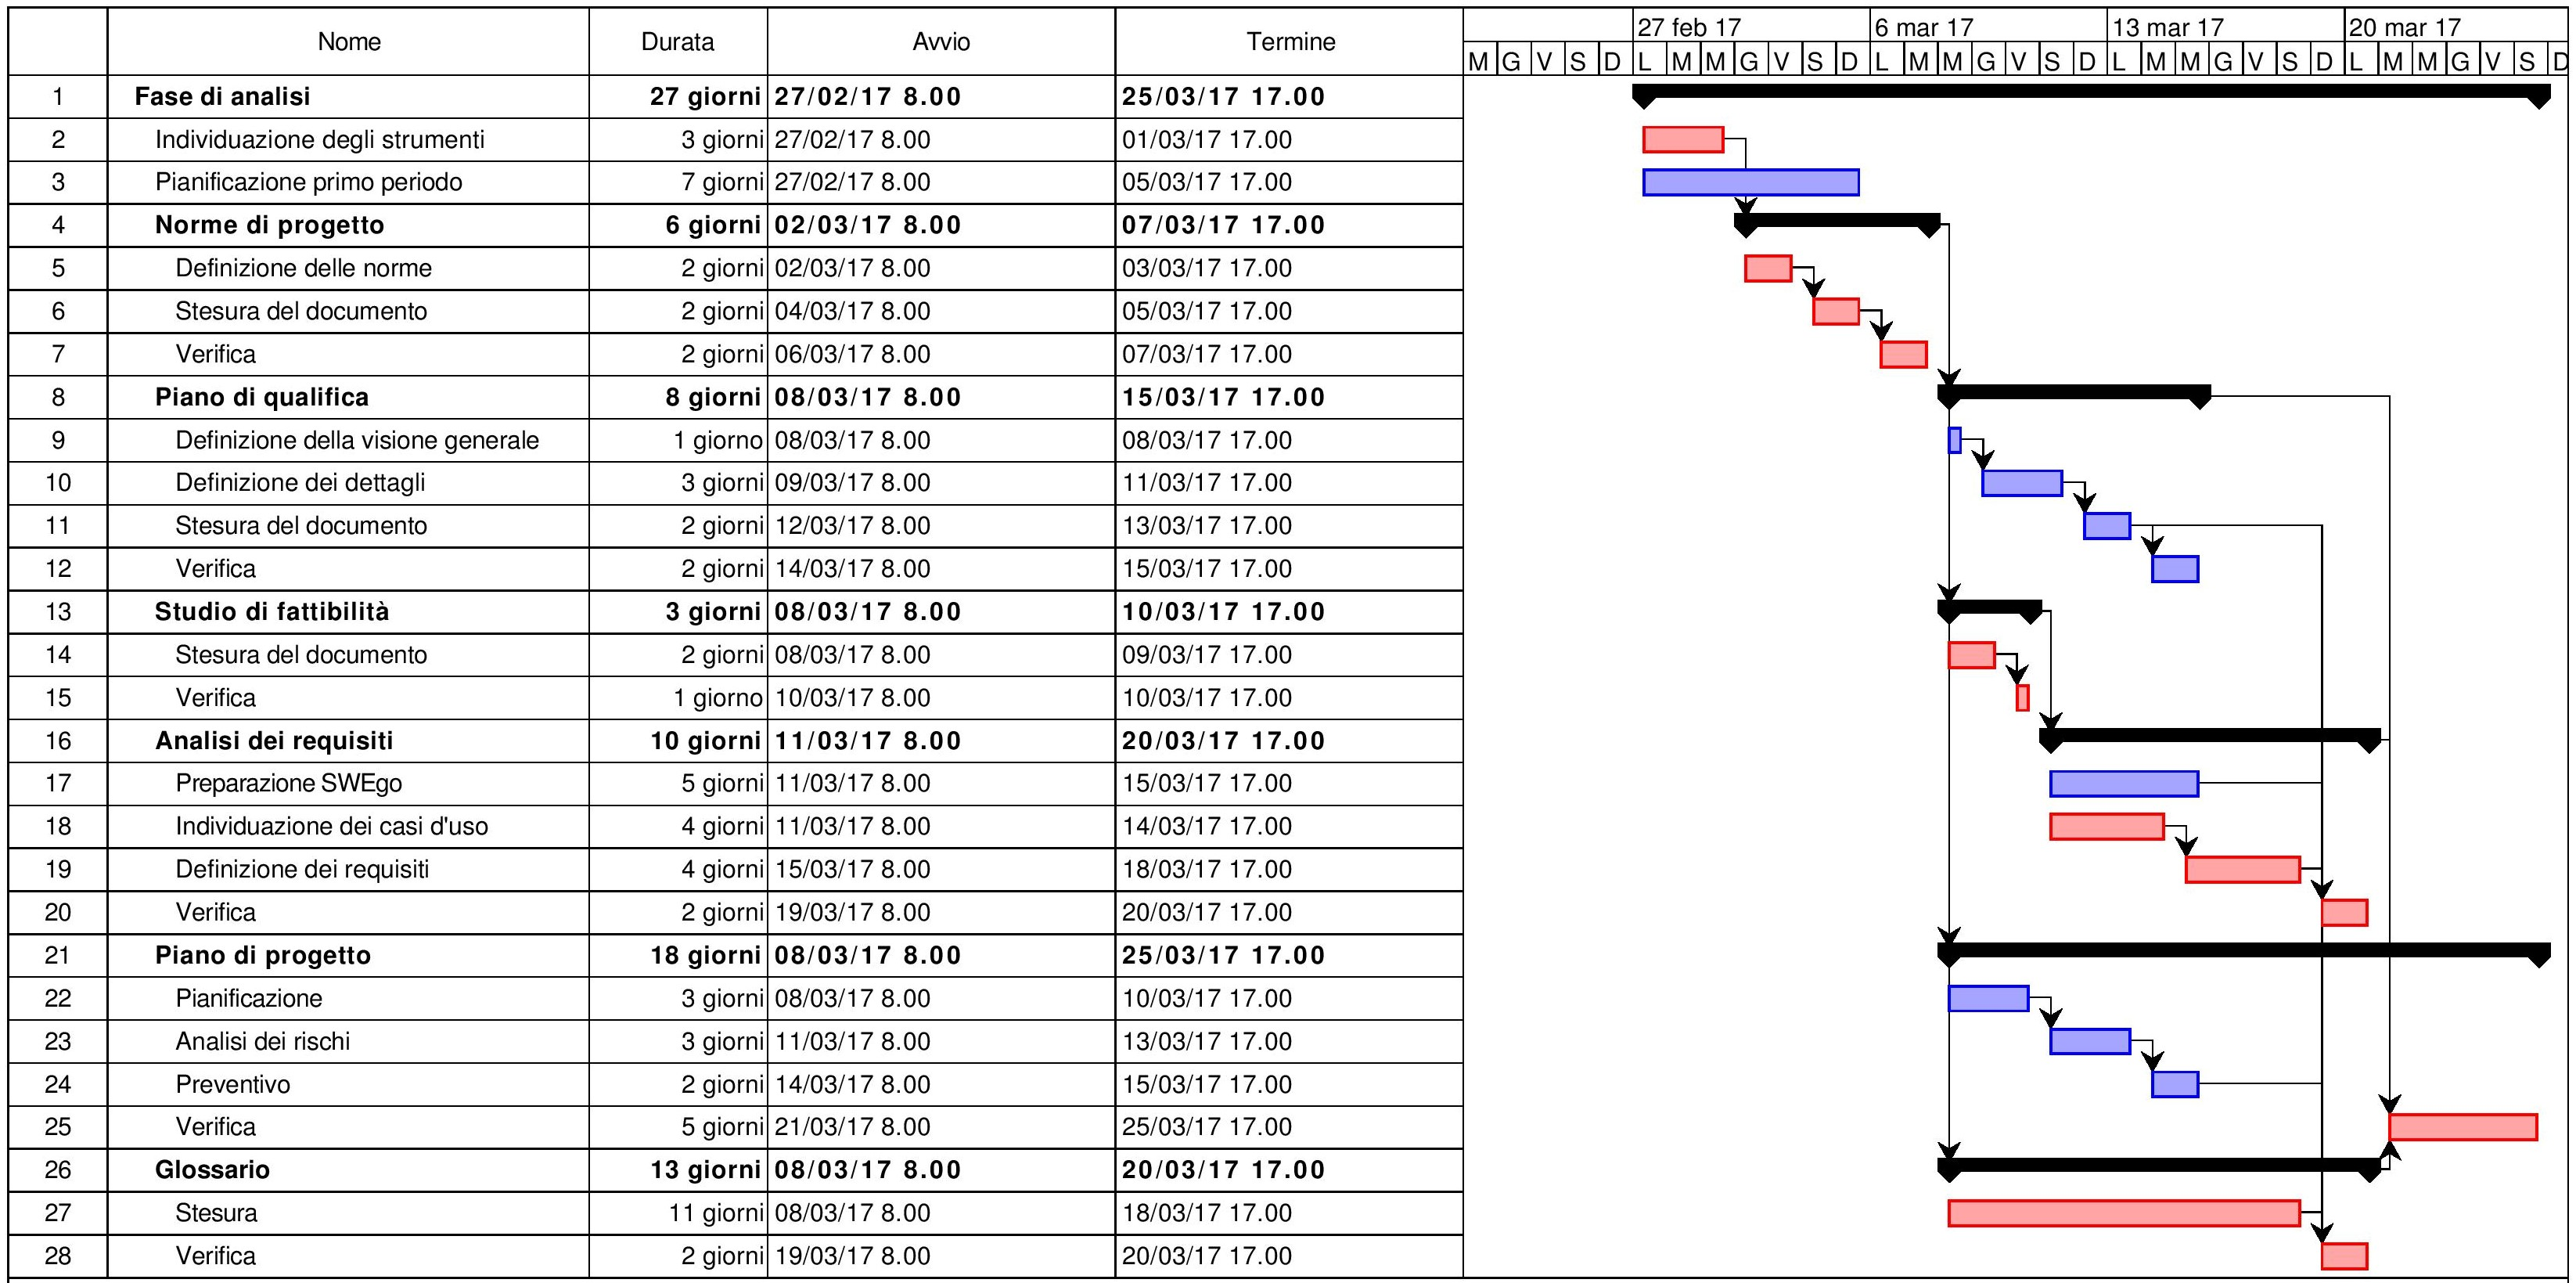
\includegraphics[scale=0.55]{Figures/Gantt_Analisi.jpg}
			\caption{Analisi: Diagramma di Gantt}
		\end{figure}
			
			
			
		\subsection{Analisi di dettaglio}
		\textbf{Periodo} : Da 26/03/2017 a 03/04/2017. \\
		Questa fase comincia con la fine della fase di analisi e prosegue fino alla scadenza della consegna della Revisione dei Requisiti.
		\begin{itemize}
			\item \textbf{Analisi di dettaglio}
			\item \textbf{Incremento e Verifica}
		\end{itemize}
		% DIAGRAMMA DI GANTT DELLE ATTIVITÀ
		\begin{figure}[H]
			\centering
			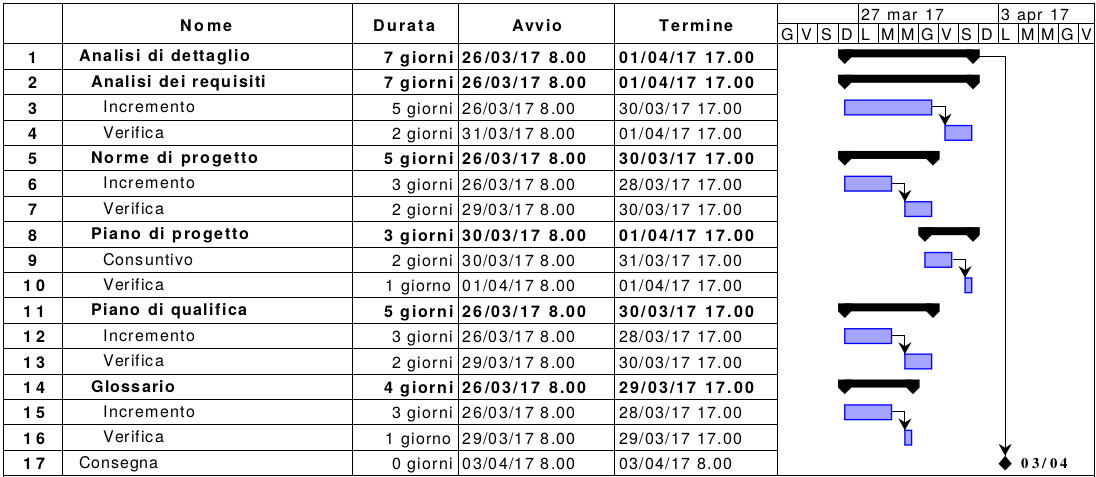
\includegraphics[scale=0.55]{Figures/Gantt_AnalisiDettaglio.jpg}
			\caption{Analisi di dettaglio: Diagramma di Gantt}
		\end{figure}
	
	
	
		\subsection{Progettazione architetturale}
		\textbf{Periodo} : Da 04/04/2017 a 27/04/2017. \\
		Questa fase comincia al termine della fase di Analisi di dettaglio e termina con un incontro di presentazione ufficiale con il proponente.
		\begin{itemize}
			\item \textbf{Specifica Tecnica}
			\item \textbf{Incremento e Verifica}
		\end{itemize}
		% DIAGRAMMA DI GANTT DELLE ATTIVITÀ
		\begin{figure}[H]
			\centering
			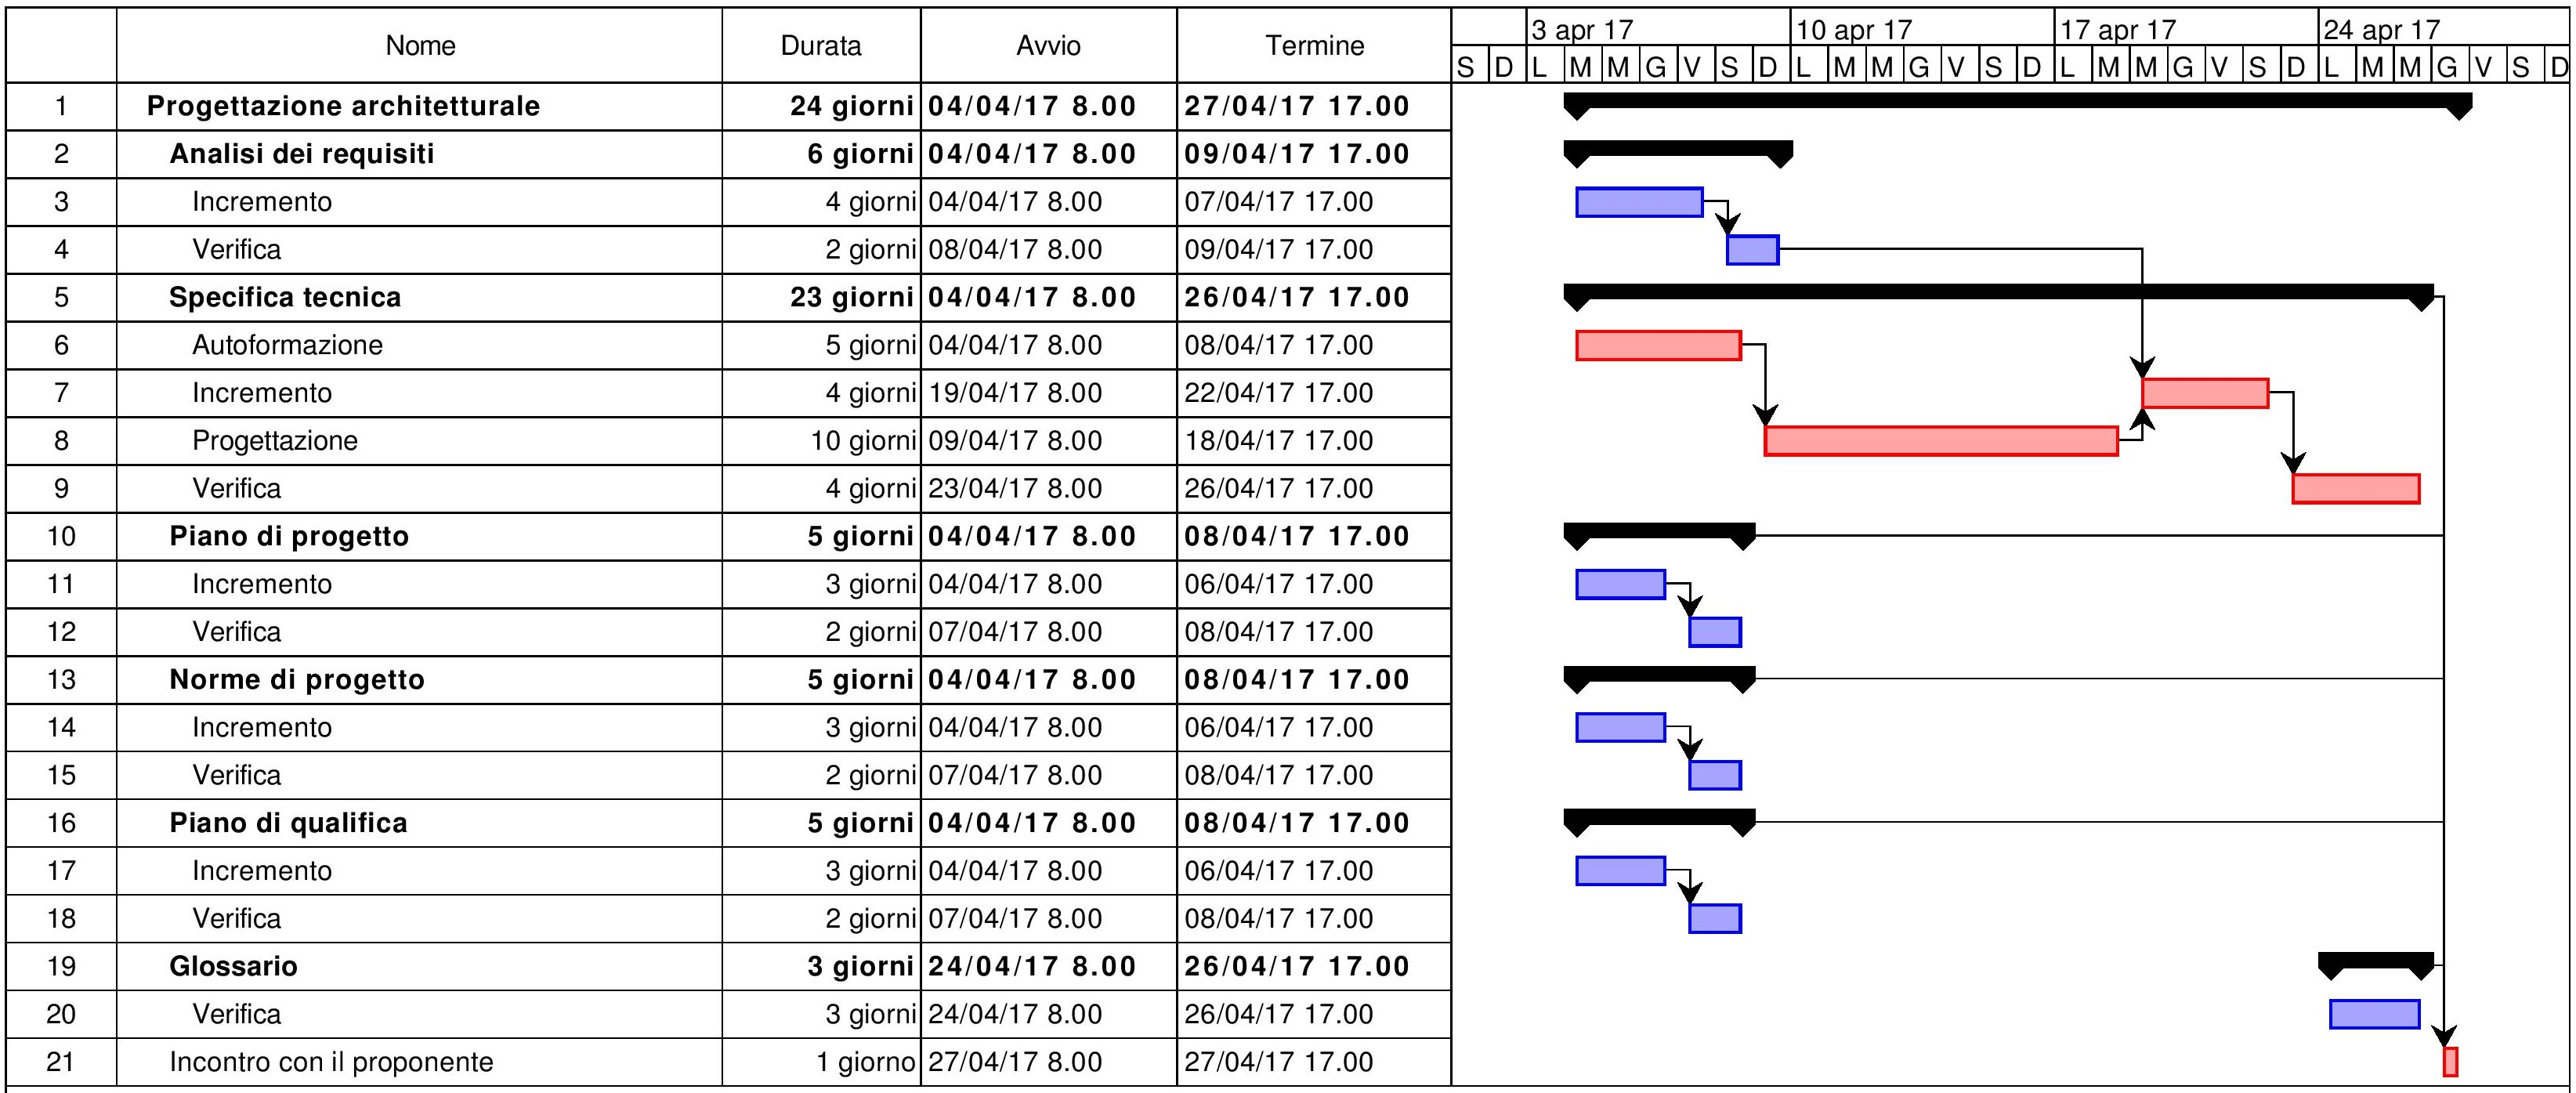
\includegraphics[scale=0.55]{Figures/Gantt_ProgettazioneArchitetturale}
			\caption{Progettazione architetturale: Diagramma di Gantt}
		\end{figure}
		
		
		
		\subsection{Progettazione di dettaglio e Codifica}
		\textbf{Periodo} : Da 28/04/2017 a 20/06/2017. \\
		Questa macro-fase comincia al termine della fase di Progettazione architetturale e prosegue fino alla scadenza della consegna della Revisione di Qualifica.
		È a sua volta divisa in 3 grandi iterazioni che riguardano Progettazione di dettaglio e Codifica rispettivamente dei requisiti obbligatori, desiderabili e opzionali.
		\begin{itemize}
			\item \textbf{Definizione di prodotto}
			\item \textbf{Manuale Utente e Manuale Amministratore}
			\item \textbf{Incremento e Verifica}
		\end{itemize}
		% DIAGRAMMA DI GANTT DELLE ATTIVITÀ
		\begin{figure}[H]
			\centering
			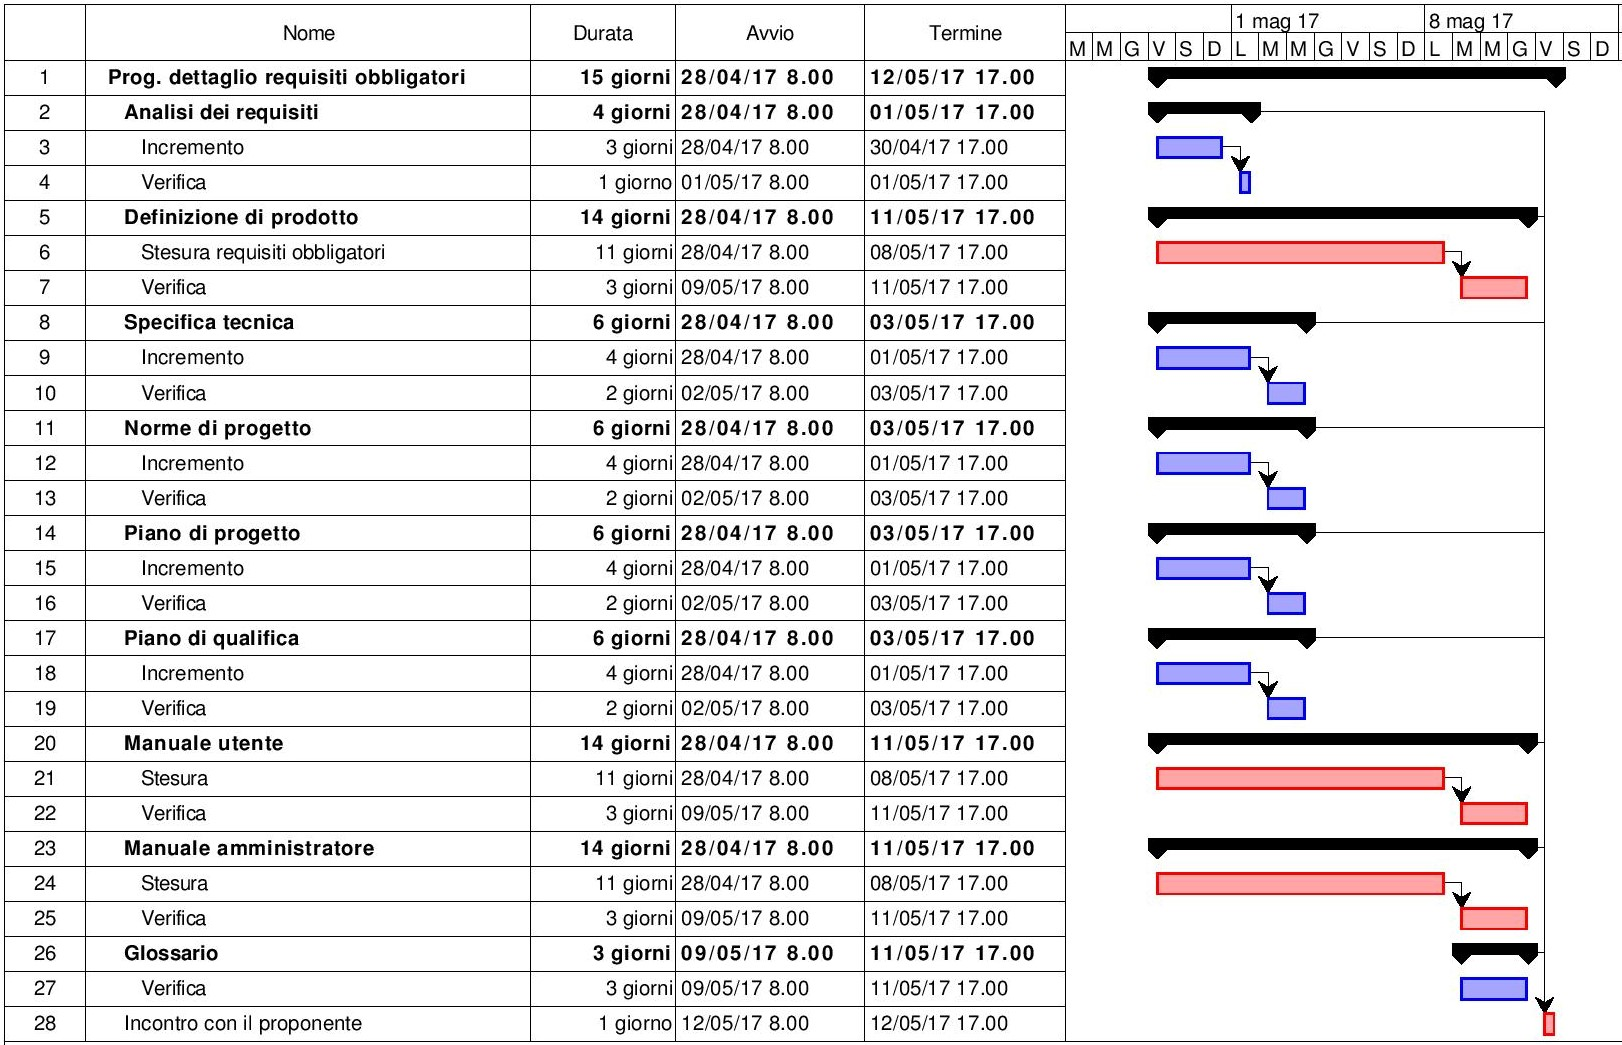
\includegraphics[scale=0.55]{Figures/Gantt_DettaglioObbligatori}
			\caption{Progettazione di dettaglio e Codifica: Diagramma di Gantt}
		\end{figure}
		\begin{figure}[H]
			\centering
			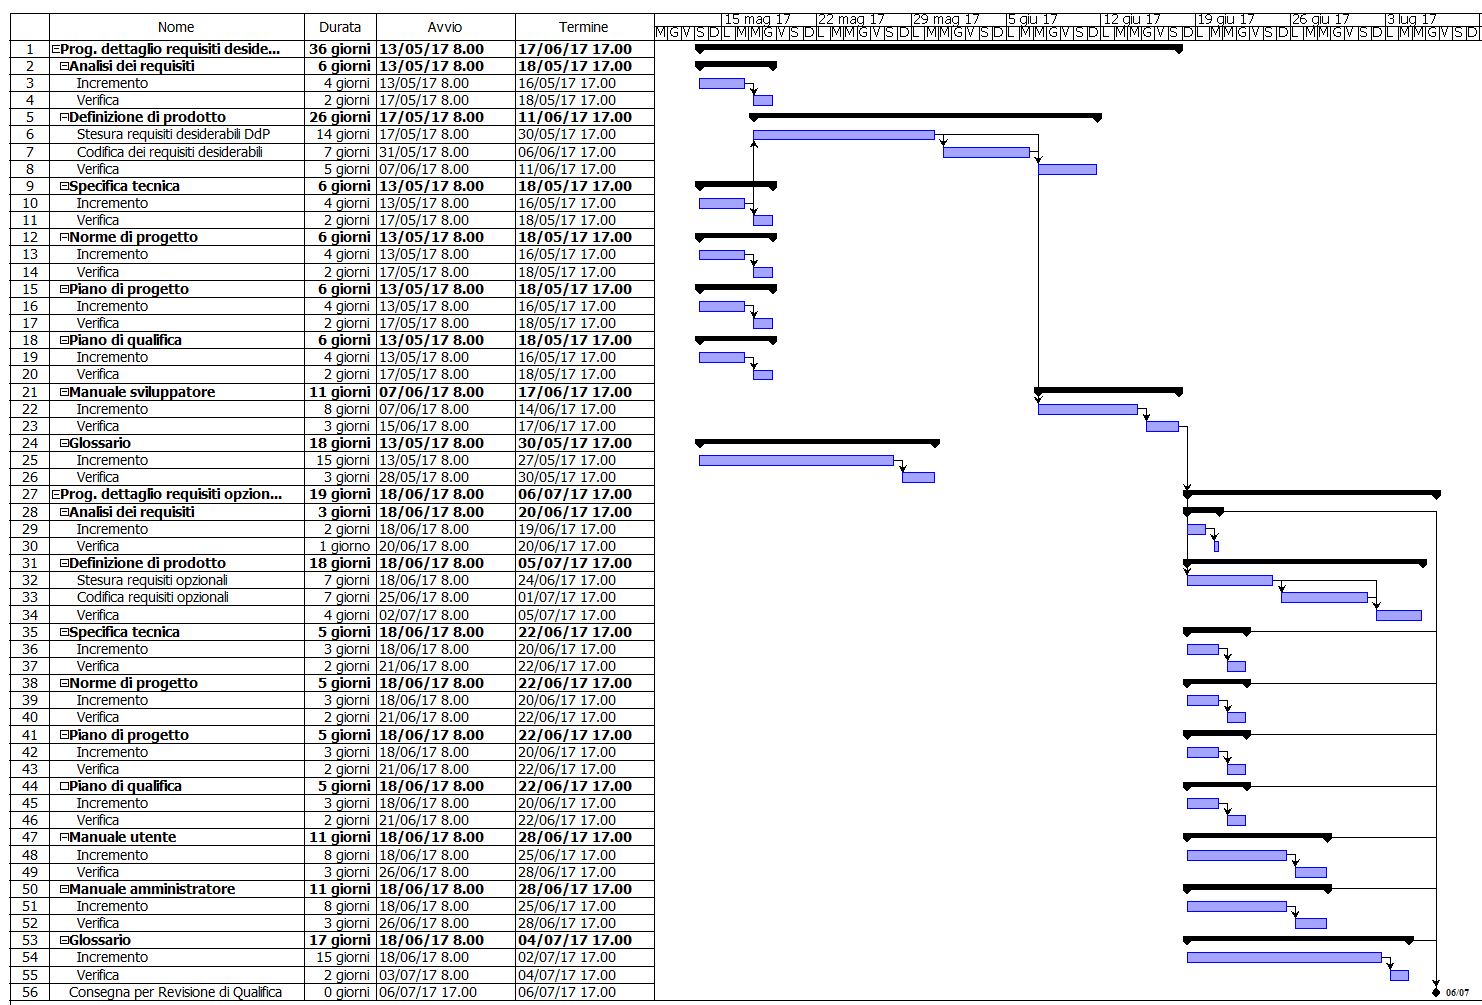
\includegraphics[scale=0.7]{Figures/Gantt_DettaglioOpz}
			\caption{Progettazione di dettaglio e Codifica: Diagramma di Gantt}
		\end{figure}
	
	
		
		\subsection{Validazione}
		\textbf{Periodo} : Da 21/06/2017 a 06/07/2017. \\
		Questa fase comincia alla fine della fase di Progettazione di dettaglio e Codifica e prosegue fino alla scadenza della consegna della Revisione di Accettazione.
		\begin{itemize}
			\item \textbf{Validazione}
			\item \textbf{Collaudo}
			\item \textbf{Incremento e Verifica}
			\item \textbf{Consegna}
		\end{itemize}
		% DIAGRAMMA DI GANTT DELLE ATTIVITÀ
		\begin{figure}[H]
			\centering
			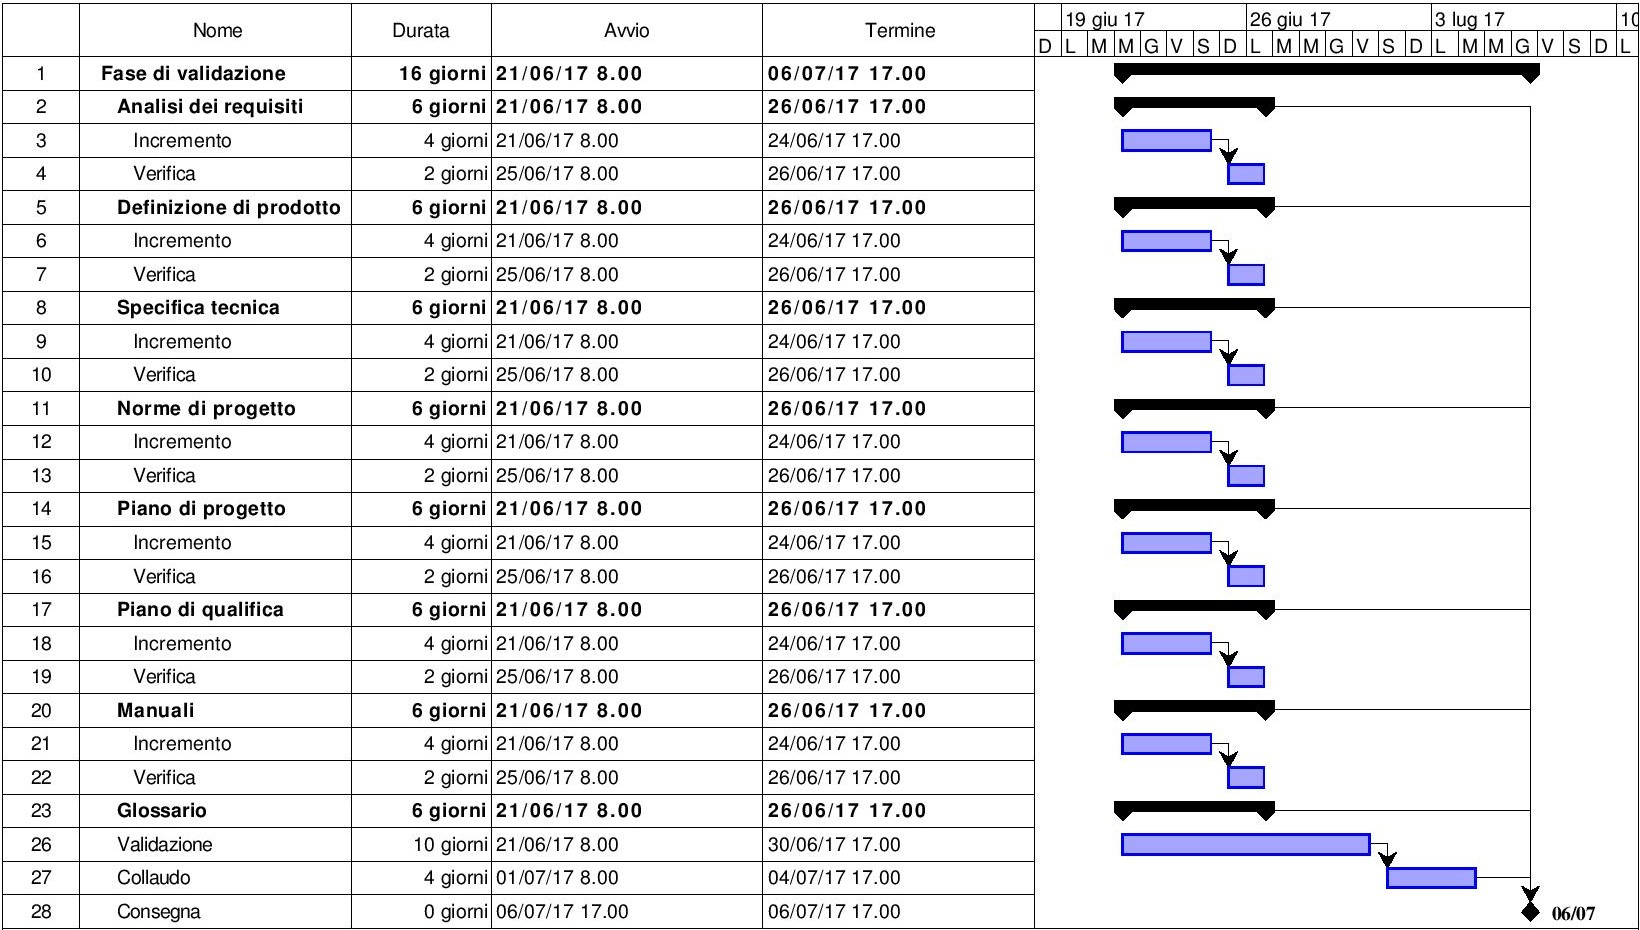
\includegraphics[scale=0.55]{Figures/Gantt_Validazione.jpg}
			\caption{Validazione: Diagramma di Gantt}
		\end{figure}
			
\end{document}
